\subsection{Implementation of temporal constraint with Huang style transfer}
In this implementation we have used the idea that style is a distribution of features described in Section \ref{sec:Style is a distribution of features}. We have utilized the Wasserstein metric in order to change the style loss of our previous implementation for style transfer for videos described in \ref{sec:Ruder style transfer}. This implementation is one of our own experiments with style transfer for video, as we combine the Ruder implementation with temporal constraint and change up the style loss to the one proposed in the paper by Huang et al. \cite{Huang:1}. 
\newline\newline
Since calculating the Wasserstein distance is computationally heavy, we have simplified this calculation. We characterize the distribution of features with simply the mean value and co-variance of the distributions, then using these to calculate the Wasserstein distance between them. For these calculations we have used TensorFlow, so we can more easily run the computations on a GPU for faster calculations.\newline\newline
The loss function for this implementation uses the same layers in the VGG-19 CNN as our implementation from Section \ref{sec:Ruder style transfer}, but the weights are different as the style loss is a lot smaller. The weight for the style loss here is 400 times larger than for our Ruder implementation. The results for this implementation can be found in Section \ref{sec:Results with wasserstein metric}.
\begin{figure}[!ht]
\begin{center}
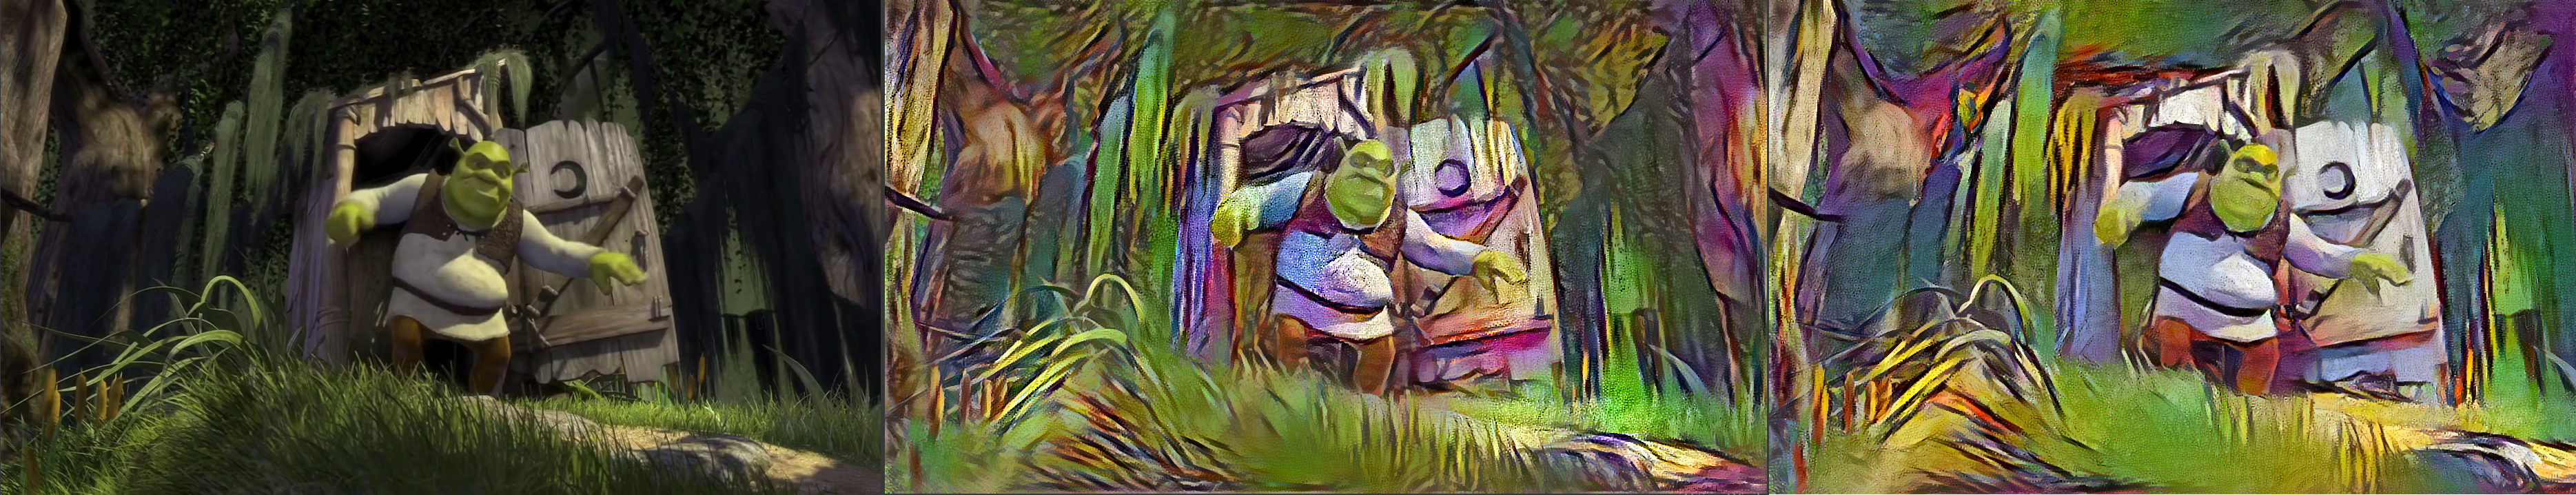
\includegraphics[scale=0.12]{report/Method/images/shrek_comparison.png}
\caption{Leftmost we see a frame from the first Shrek movie. The middle image is styled with the Gram Matrices from Gatys paper. The rightmost image is styled with Wasserstein as loss function. Both were styled with La Muse (Picasso) as style reference.}
\label{fig:architecture}
\end{center}
\end{figure}